\section{General Idea}
\label{sec:idea}


\begin{figure*}
\centering
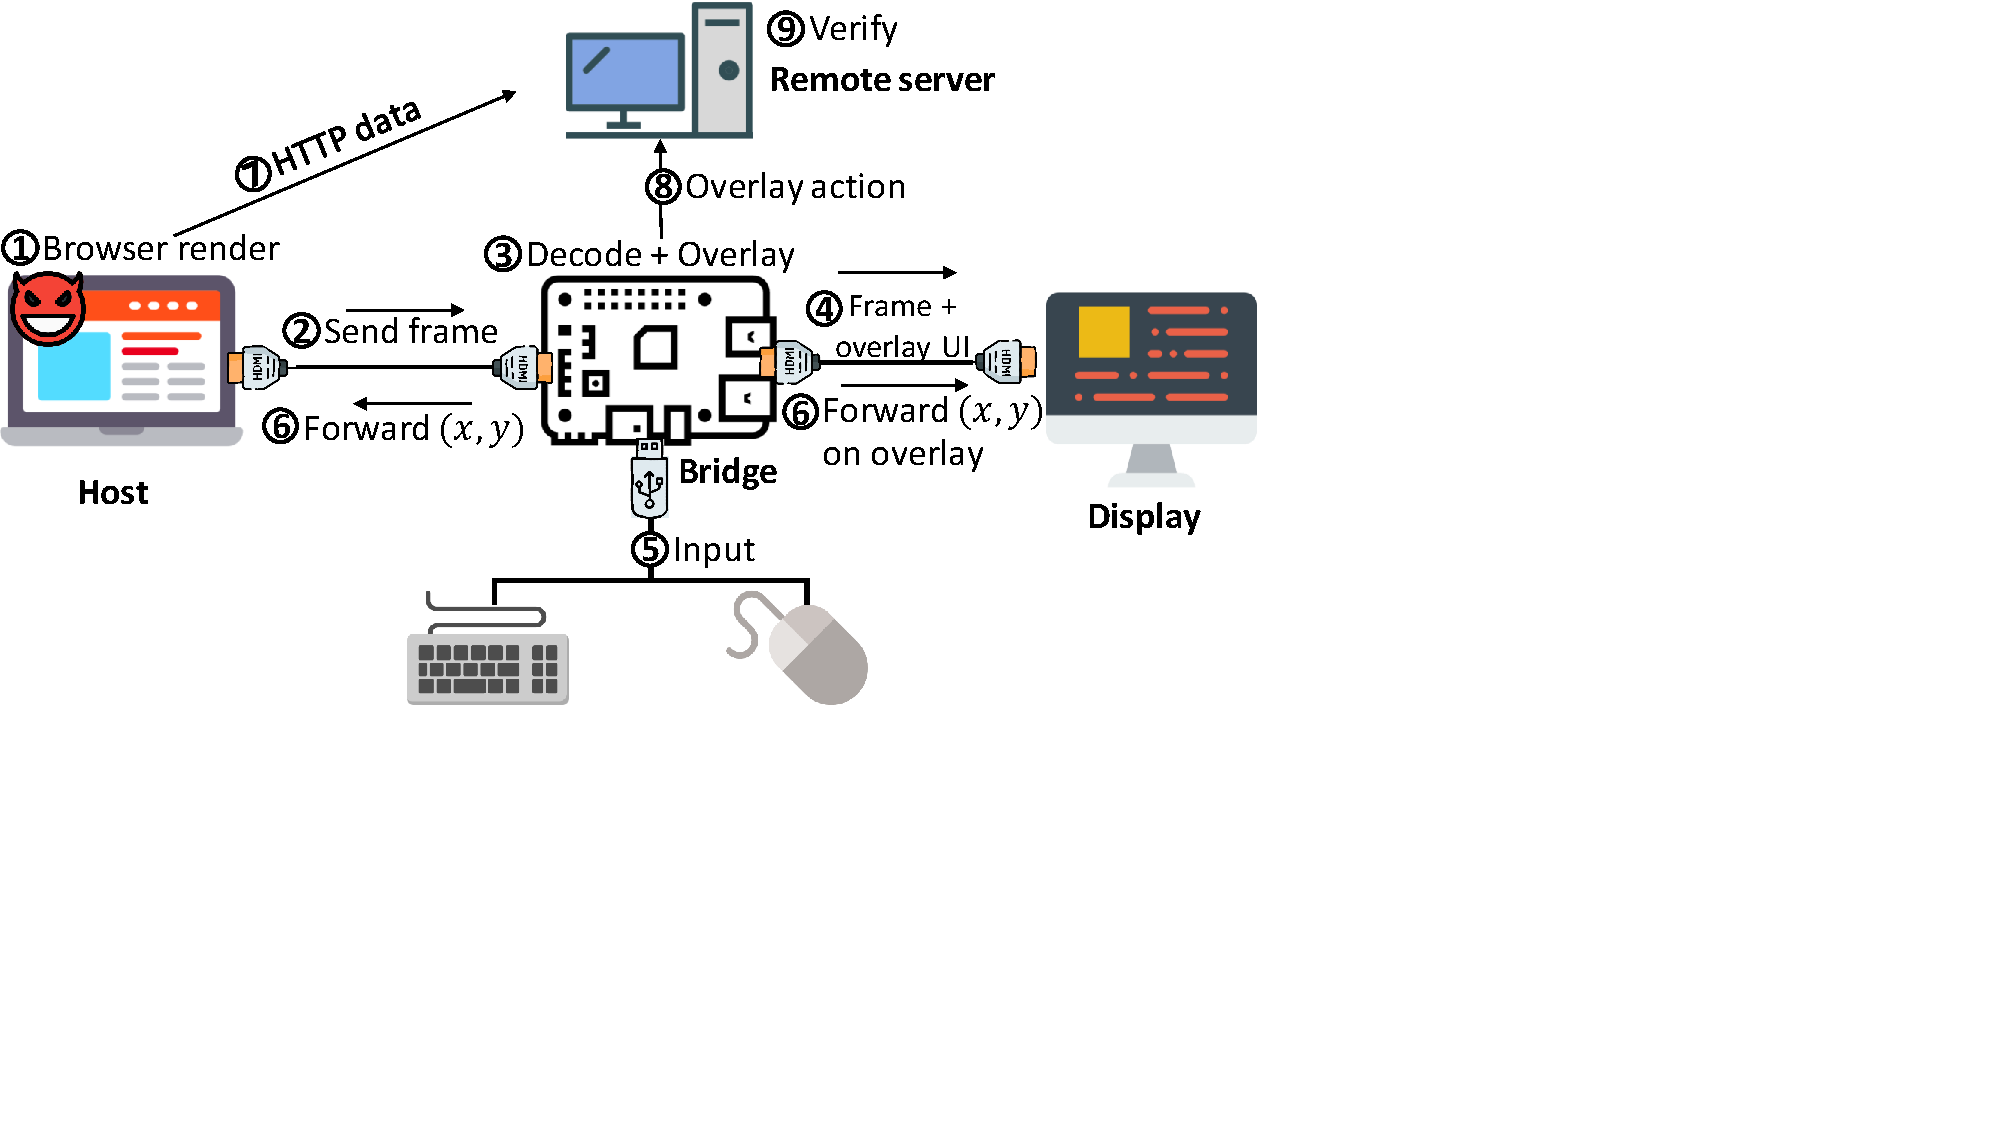
\includegraphics[trim={0 5.8cm 8cm 0}, clip, width=0.8\linewidth]{systemDesign.pdf}
\caption{System Design}
\label{fig:systemDesign}
\centering
\end{figure*}

% \begin{figure}
% \centering
% 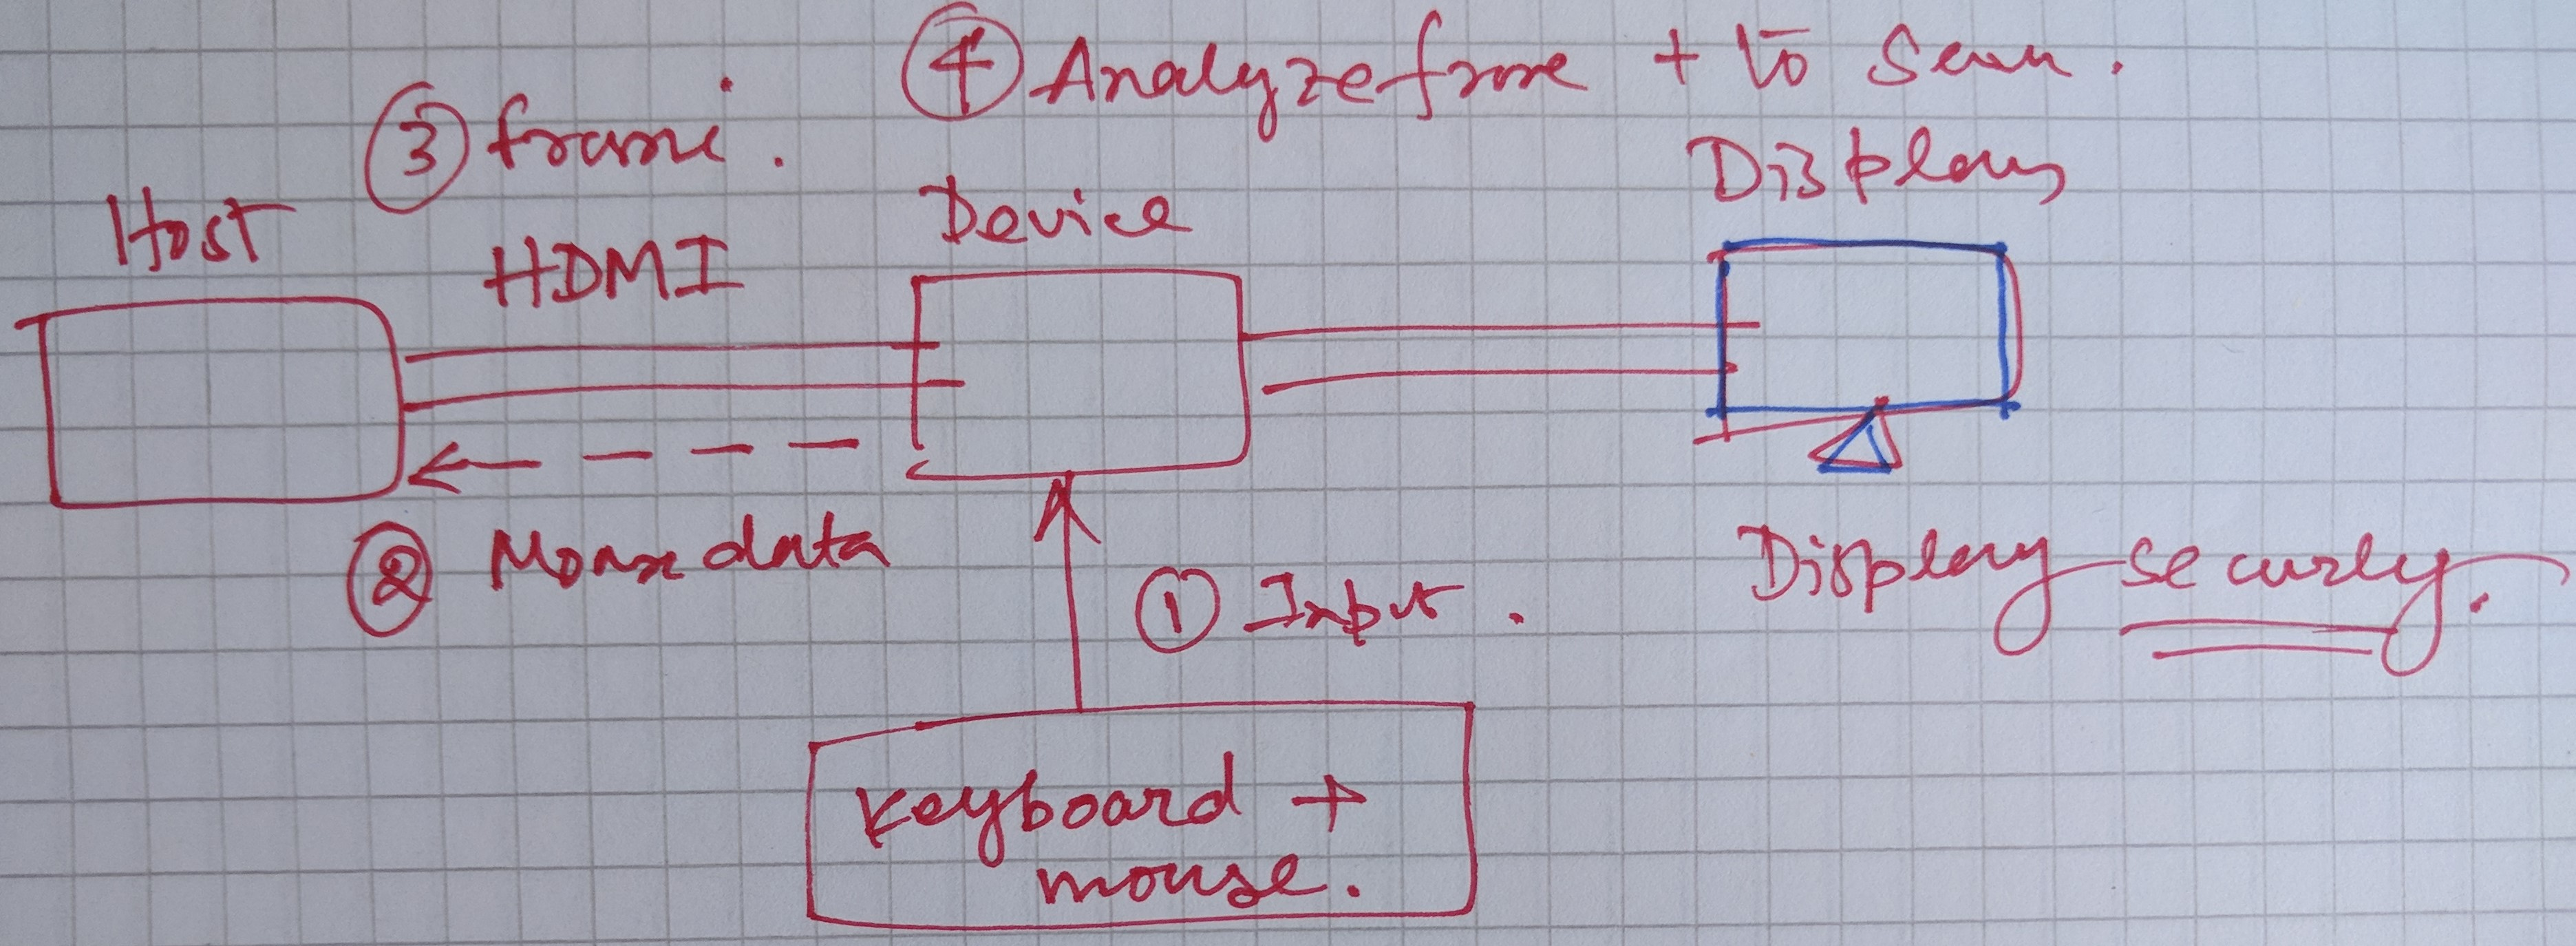
\includegraphics[width=\linewidth]{overall.jpg}
% \caption{Overall idea}
% \label{fig:overallIdea}
% \centering
% \end{figure}

Figure~\ref{fig:systemDesign} provides the overall system design of \name. The components of the systems are the following:

\begin{enumerate}
  \item \textbf{\device.} The \device is connected to the input devices and sits between the host and the display. The \device is connected to the input devices over \usb interface and connected to the host and the display over HDMI.
  \item \textbf{Input device.}
  \item \textbf{Display.}
  \item \textbf{Host system.}
\end{enumerate}

\myparagraph{Initialization} The \device initializes the mouse by instructing the host system to move the mouse pointer to top right corner (moving to the first right and then up for an arbitrarily large value). As the \device has access to the frames that are displayed on the screen, it can verify if the mouse pointer is at the top-right corner of the screen or not. Then it instructs the host OS to bring it to the center of the screen.

The steps are the following:

\begin{enumerate}
  \item The user provides input from her input device which is captured by the \device.
  \item The \device sends the mouse traces to the host over the \bluetooth interface.
  \item The host system draws the frames and send it to the \device over HDMI interface.
  \item The device analyzes (Section~\ref{sec:idea:analysis}) the frames passed from the host system. Then it sends the frames to the display over HDMI.
\end{enumerate}


\begin{figure}
\centering
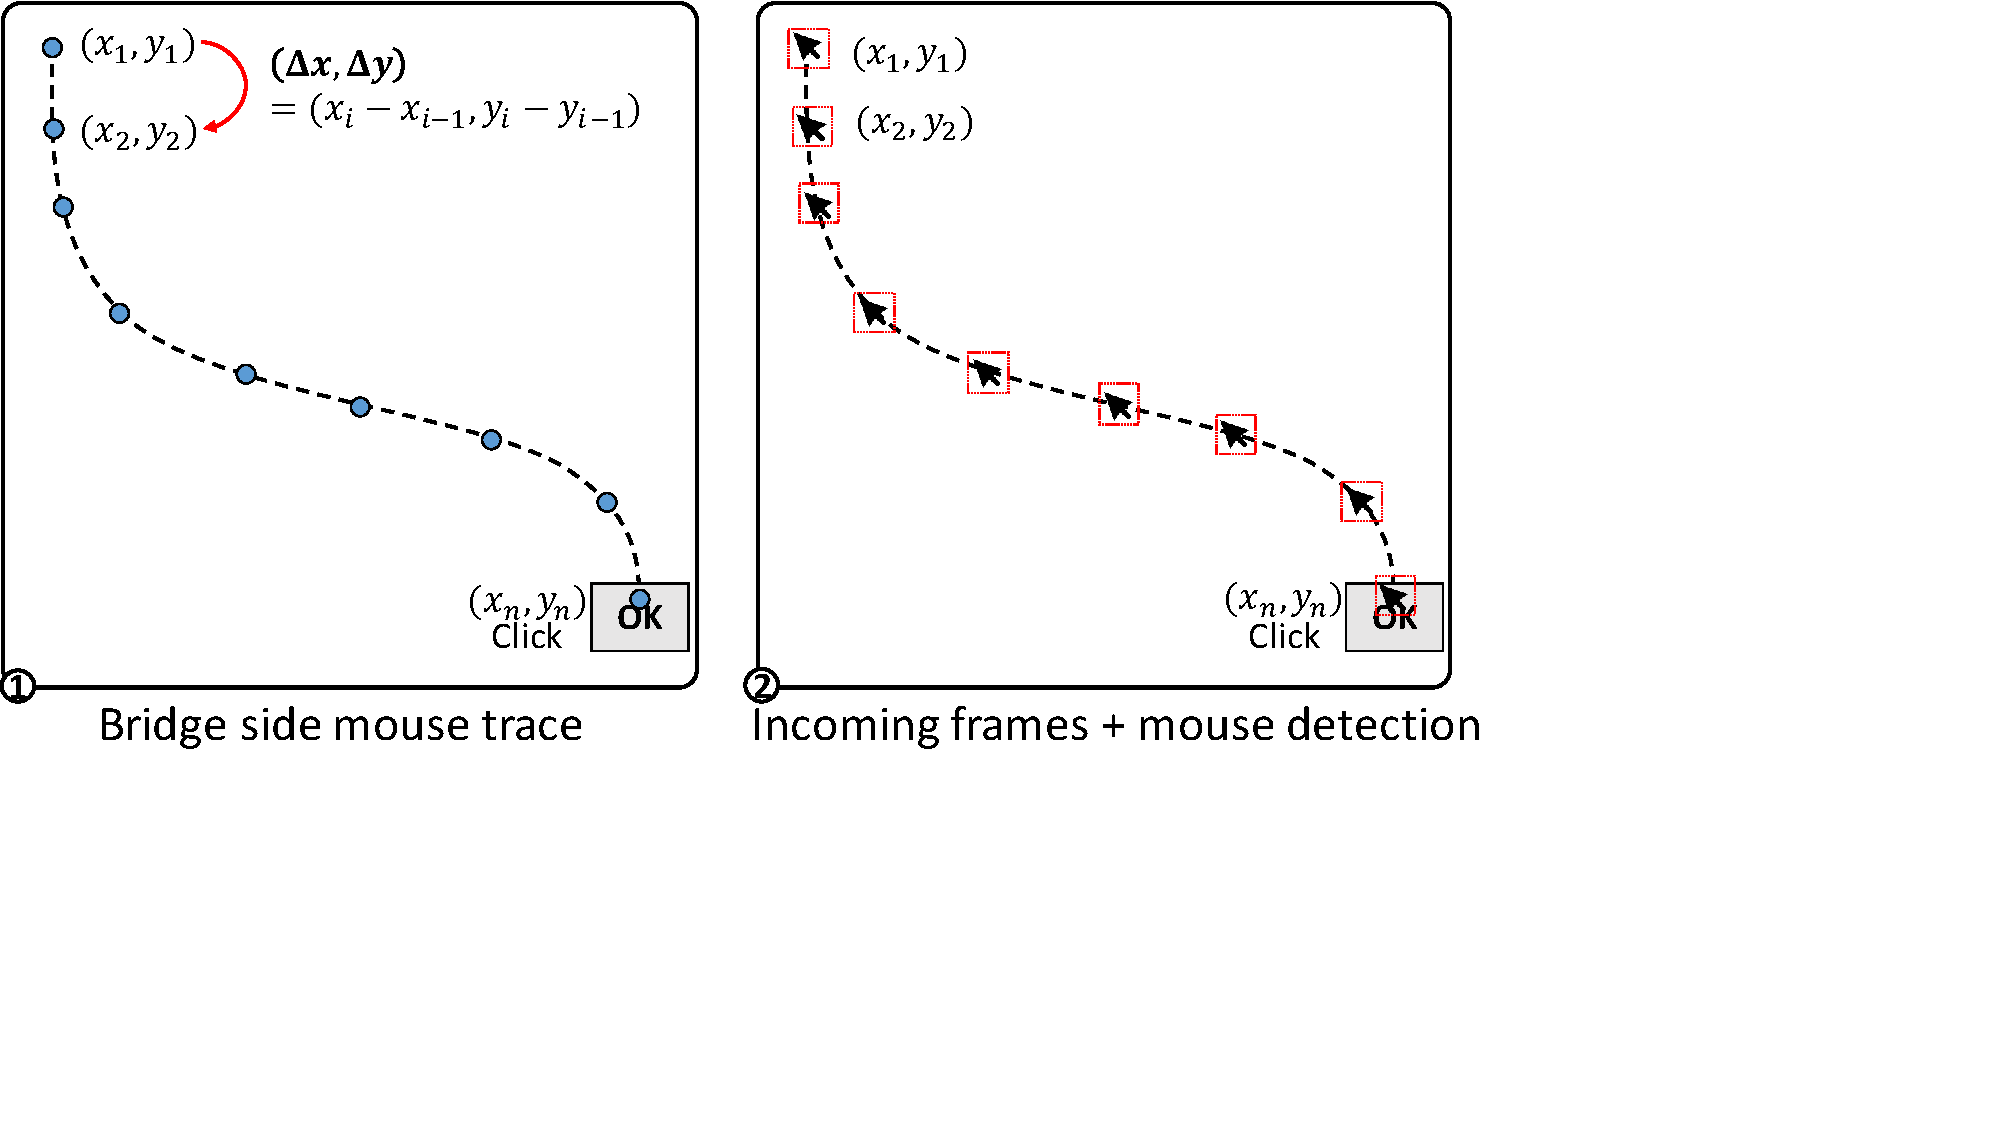
\includegraphics[trim={0 5.8cm 8cm 0}, clip, width=\linewidth]{mouseAnalysis.pdf}
\caption{Analysis of the frames in comparison with the mouse trace}
\label{fig:mouseAnalysis}
\centering
\end{figure}

% \begin{figure}
% \centering
% 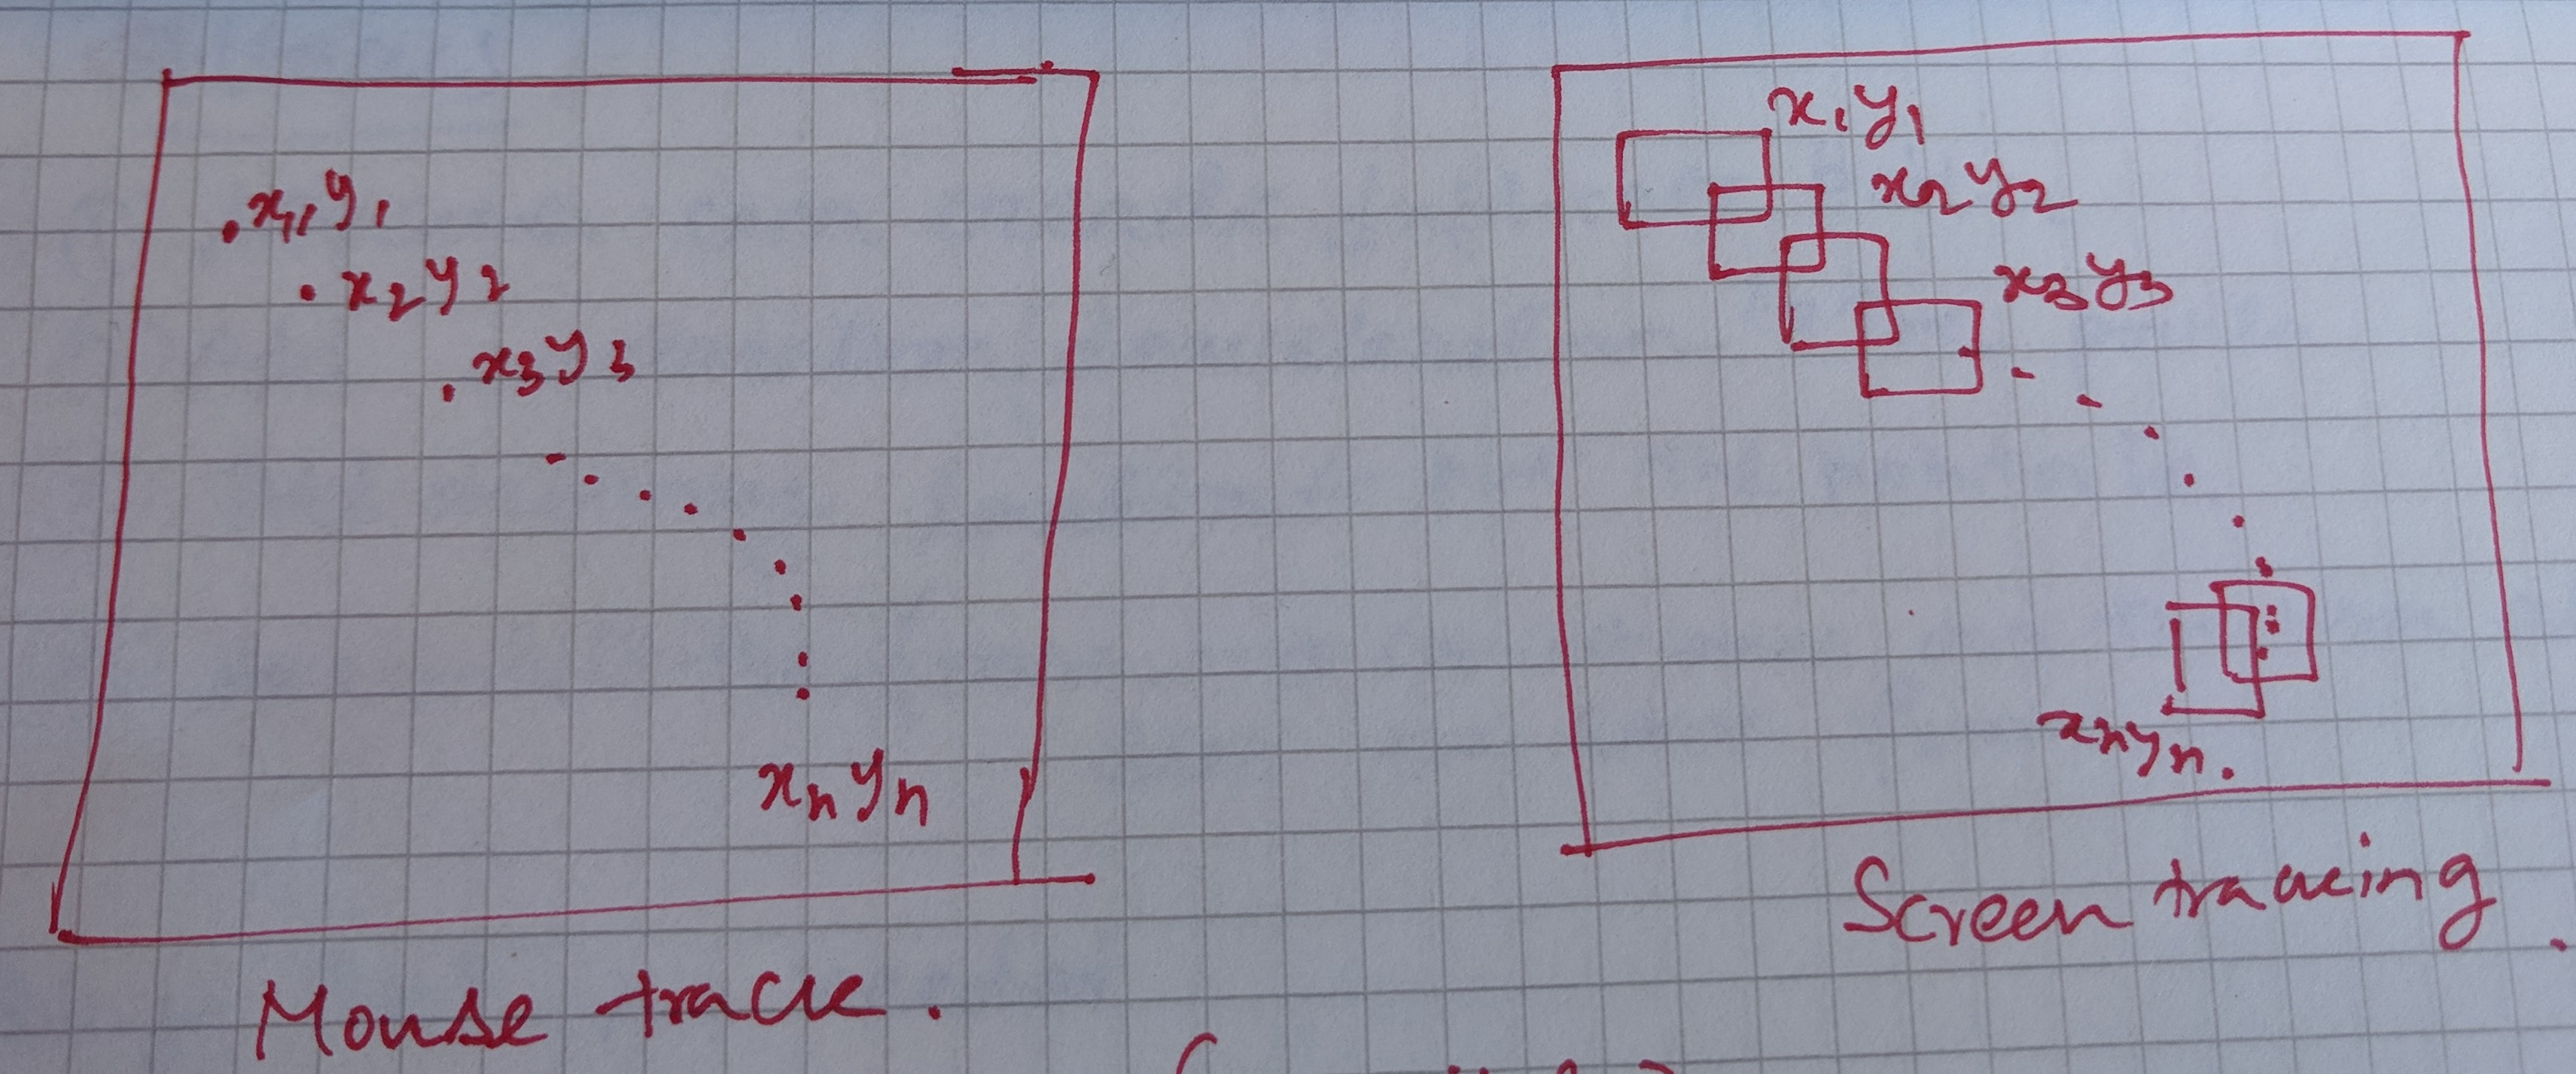
\includegraphics[width=\linewidth]{mouse_track.jpg}
% \caption{Analysis of the frames in comparison with the mouse trace}
% \label{fig:mouseAnalysis}
% \centering
% \end{figure}

\subsection{Analysis of host frames}
\label{sec:idea:analysis}

Figure~\ref{fig:mouseAnalysis} illustrates the high-level idea of the host system display frame analysis. To match the mouse polling rate with the display frame rate, the \device only queries the input device with the frequency of $60$ Hz. We assume that over the HDMI channel the host system sends frames at the rate of $60$ fps. The analysis works like the following. We define mouse movement as the time series $(x,y)$ co-ordinates $\{(x_1,y_1), (x_2, y_2), \ldots, (x_n,y_n)\}$ from time $\{t_1, t_2, \ldots, t_n\}$. Assume that the frames coming from the host system to the \device are: $\{f_1, f_2, \ldots, f_n\}$. In time $t_i$, the \device looks into the frame $f_i$ and draws a square centered at $(x_i, y_i)$ with sides of length $X$ (enough to cover a mouse cursor). Then the \device checks if there exists a mouse inside this square or not. In case there exists a mouse cursor, the \device allows further user interactions otherwise it stops all the communications and shows an error on the display.

\begin{figure}
\centering
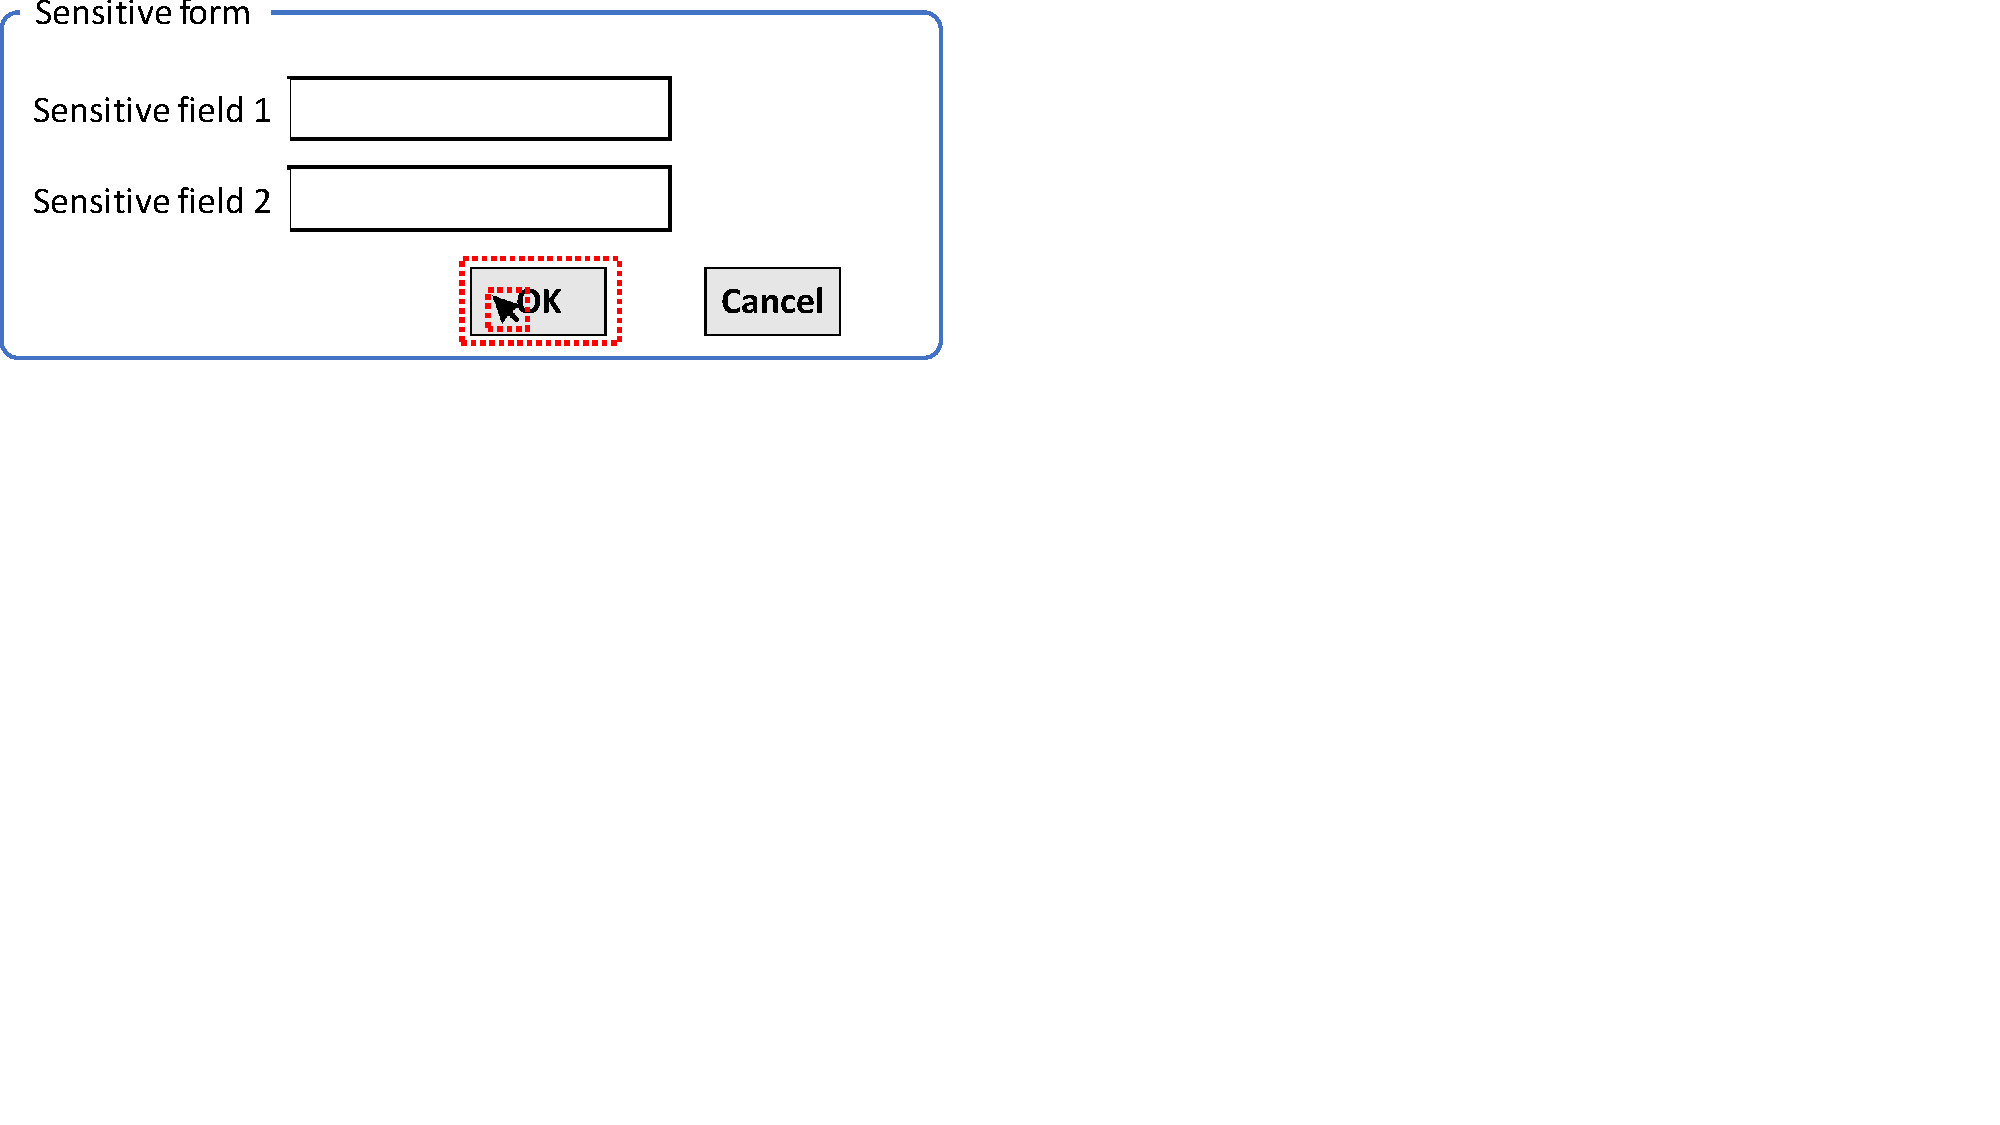
\includegraphics[trim={0 12cm 17cm 0}, clip, width=0.8\linewidth]{uiDetect.pdf}
\caption{Detection of the UI elements upon mouse click event in the incoming frame.}
\label{fig:uiDetect}
\centering
\end{figure}

% \begin{figure}
% \centering
% 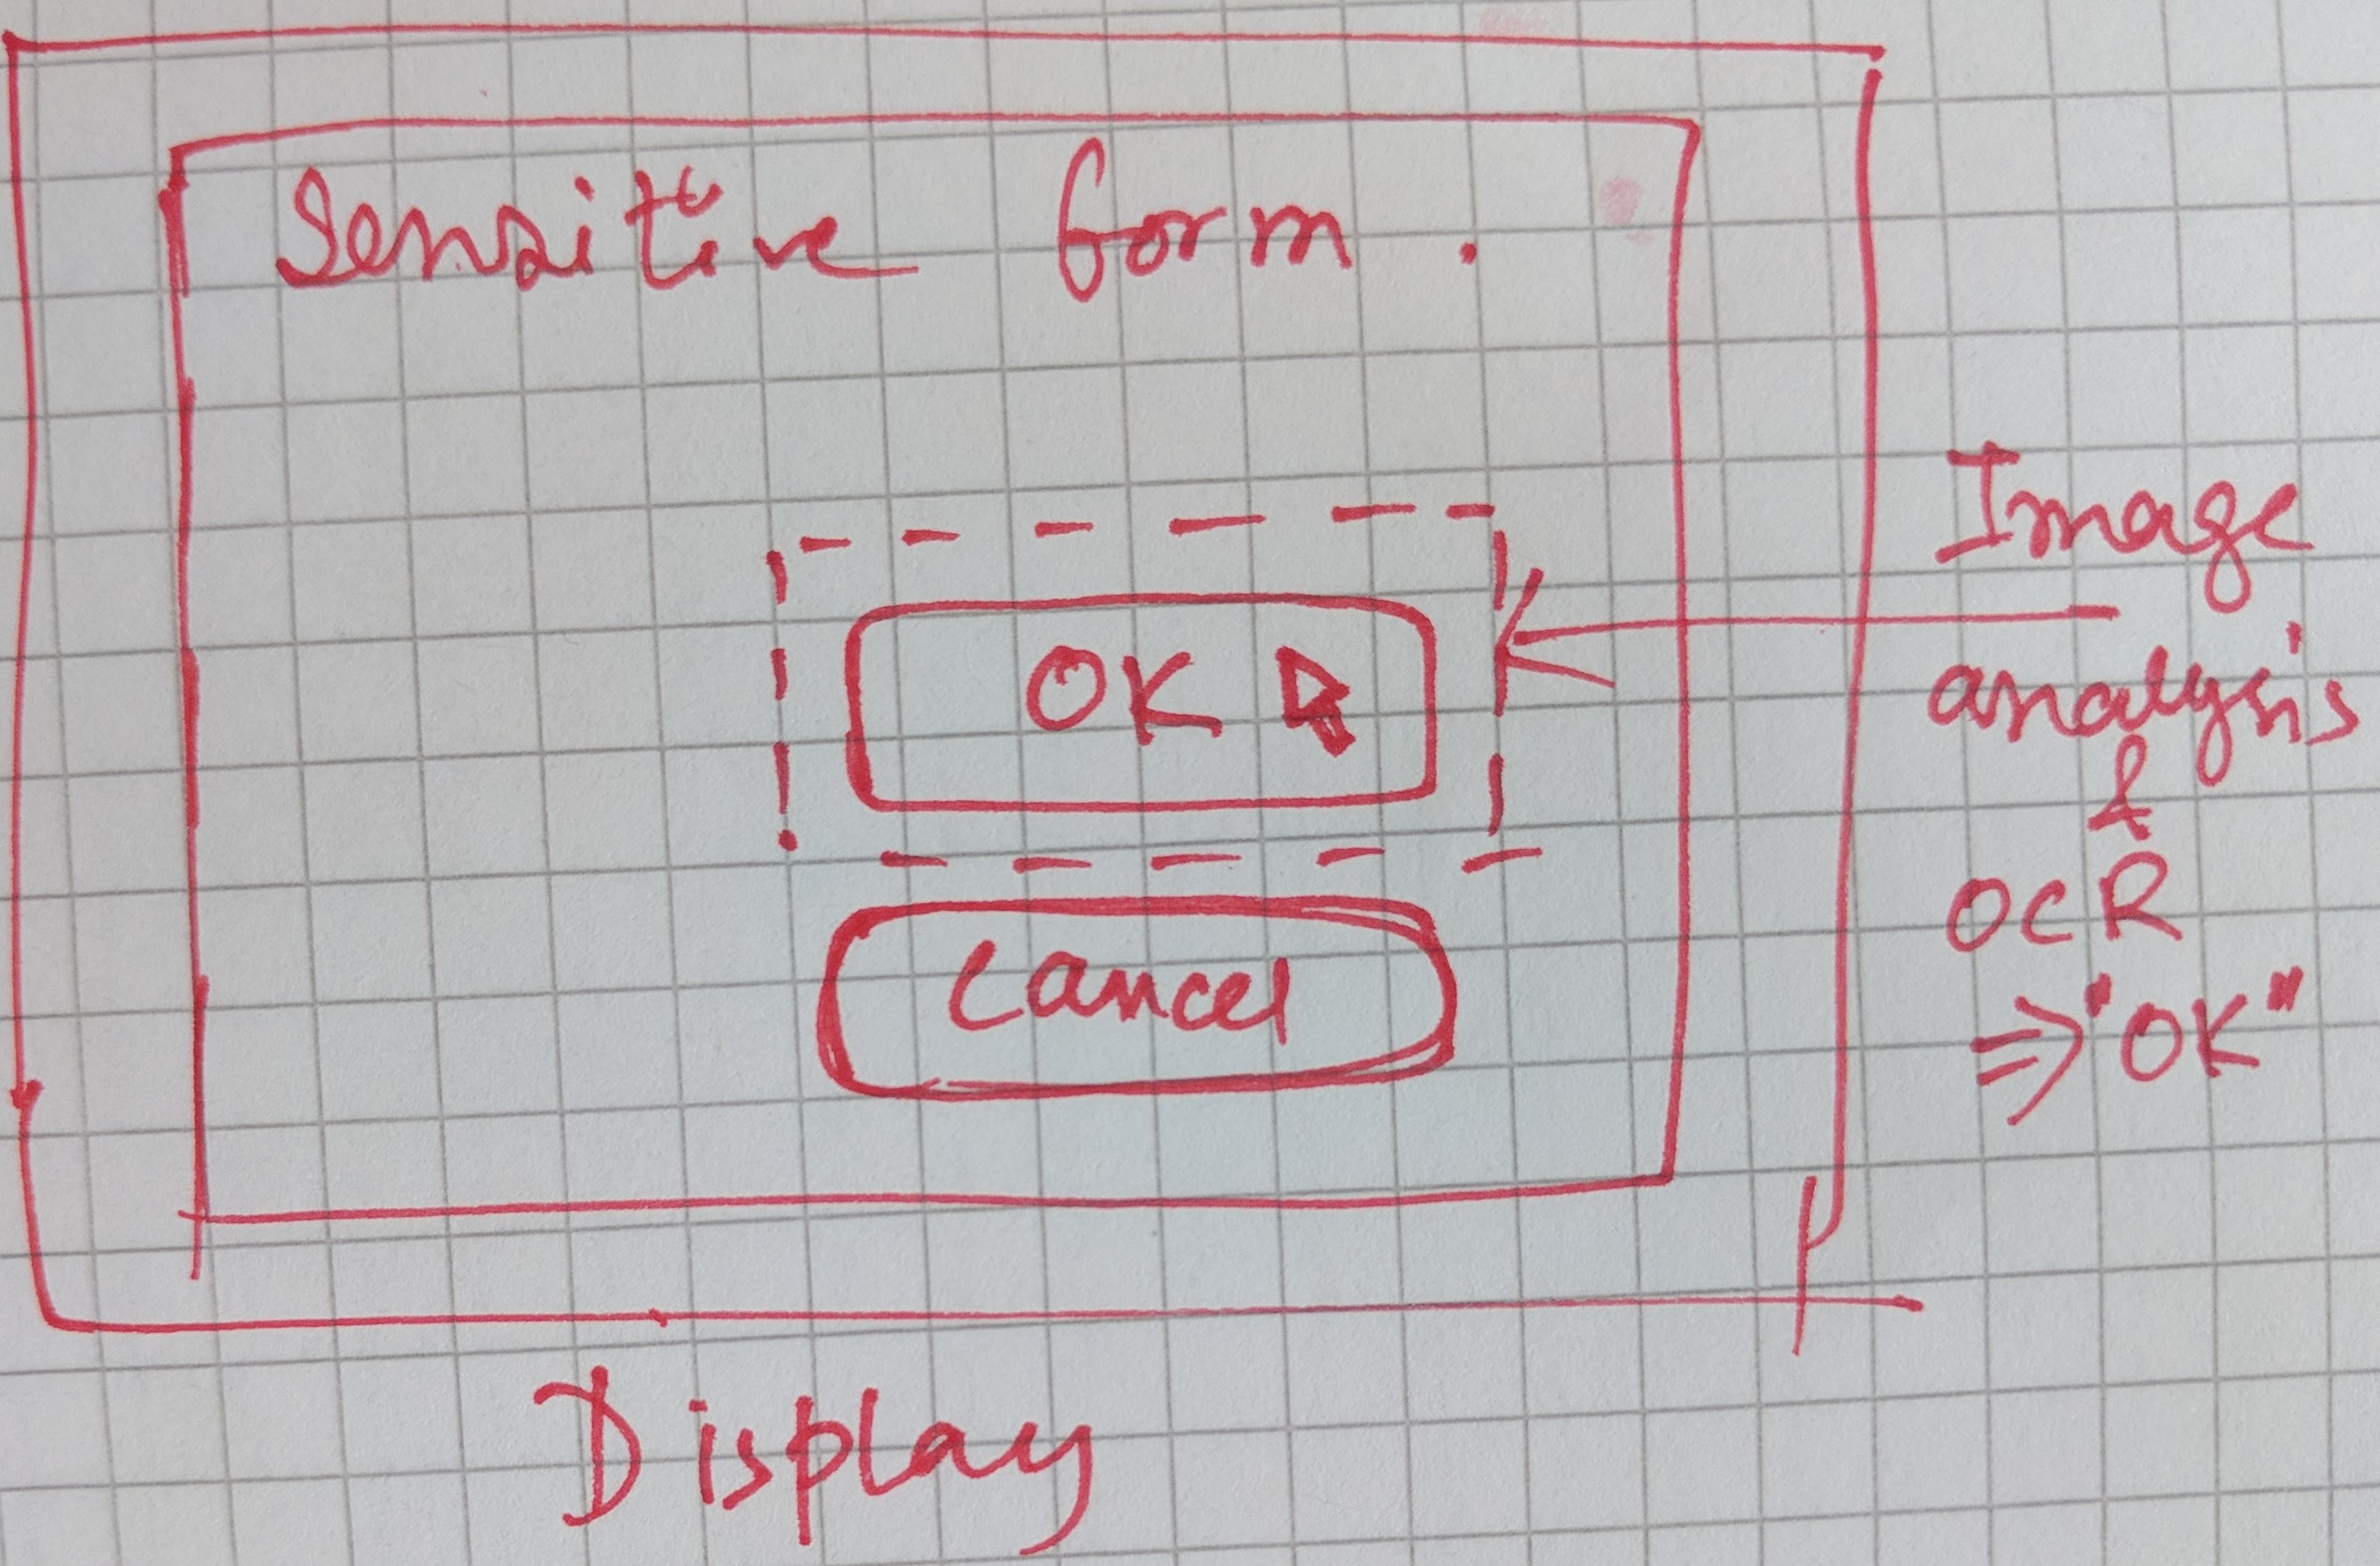
\includegraphics[width=\linewidth]{ui_detect.jpg}
% \caption{Detection of UI elements}
% \label{fig:uiDetect}
% \centering
% \end{figure}

\subsection{Detecting UI elements}

Detecting the UI elements triggers when the user clicks. The \device uses a square of $X$ sq. pixels around the mouse pointer and analyze the image. For example, if the user clicks on a button, the \device executes the image analysis on the part of the image to try to figure out if there is a button and parse the text. Additionally, the \device also sends the button text to the server. The server checks the data sent by the \device and the data received from the browser and compares them. In case there is a mismatch, the server notifies the \device and the \device overlays an error message on the screen. 


